% !TeX spellcheck = de_CH_frami

\section{Frequenzverhalten von MOS-Verstärkern (Kap. 11)}
\subsection{Analyse mittels Open-Circuit Time Constant Methode} 
\begin{minipage}[c]{0.5\textwidth}
	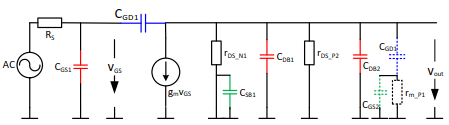
\includegraphics[width=1\linewidth]{chapters/Frequenzverhalten/images/parasitaere_kapazitaeten}
\end{minipage}
\begin{minipage}[c]{0.5\textwidth}
\textbf{Bestimmung des für die Bandbreite verantwortlichen Pols:}
\begin{compactenum}
	\item Setze alle unabhängigen Quellen = 0 (V $\rightarrow$ Kurzschluss, I $\rightarrow$ Leerlauf)
	\item Berechne für alle Kapazitäten die zugehörige Zeitkonstante, wenn alle anderen C = 0.
\end{compactenum}
\end{minipage}
\begin{compactenum}
	\setcounter{enumi}{2}
	\item Bestimme die Bandbreite als Summe der Zeitkonstanten: $\omega_{-3dB}\approx \frac{1}{\sum\tau_k}=\frac{1}{\sum R_kC_k}$
\end{compactenum}
Frequenz des dominierenden Pols $f_d$ und somit die Bandbreite: $f_d=\frac{1}{2\pi \cdot R_dC_d}$\\
\textbf{Vorgehen für Frequenzanalyse:}
\begin{compactenum}
	\item DC Verstärkung berechnen (aus Kleinsignalersatzschaltung für tiefe Frequenzen)
	\item Die für die Übertragungsfunktion relevanten Pole (und Nullstellen) des	Systems finden. Frage: An welchem Knoten befinden sich gleichzeitig ein hoher Widerstand und eine grosse Kapazität, also ein grosses RC-Produkt.
	\item Einzeichnen der einzelnen Pole (und allenfalls Nullstellen) ins Bode-Diagramm.
\end{compactenum}
Für eine grobe Analyse des Frequenzverhaltens genügt es somit, die Knoten zu suchen, bei denen das grösste RC-Produkte auftritt. Dort wird der dominierende Pol entstehen, welcher einen Abfallen des Frequenzgangs um 20dB/Dekade einleiten.
\subsection{Widerstände}
\begin{tabular}{lll}
	Knotenimpedanz praktisch unendlich: &$r_{iG}\rightarrow \infty$ & Gate \\
	Knotenimpedanz sehr hoch: &$r_{ds} = \frac{1}{g_0}$ & Drain wenn Stromquelle\\
	Knotenimpedanz tief: &$\frac{1}{g_m}$ & Drain wenn Diodenschaltung, Source wenn Stromquellenschaltung \\
\end{tabular}
\subsection{Kapazitäten}
